\chapter{Теоретические основы Retrieval-Augmented Generation}
\label{chapter:theory}

\section{Большие языковые модели}

Большие языковые модели предназначены для обработки и генерации текста на естественном языке. Современные LLM основаны на архитектуре Transformer, в которой механизм внимания позволяет учитывать связи между токенами во входной последовательности~\cite{Vaswani2017Attention}. В прикладных задачах такие модели используются для ответа на вопросы, суммаризации, классификации, преобразования текста и диалогового взаимодействия.

Ответ LLM существенно зависит от переданного контекста и инструкции. Если модель получает только вопрос, она опирается на знания, зафиксированные в параметрах во время обучения. Для внутренних корпоративных документов это является ограничением: материалы могут отсутствовать в обучающем наборе, быть обновлены после обучения модели или содержать специфические термины. В таких условиях возможны галлюцинации, то есть правдоподобные, но неподтвержденные утверждения.

В RAG-сценарии LLM используется не как самостоятельный источник знаний, а как генератор ответа по найденному контексту. Это не устраняет все возможные ошибки, но позволяет ограничить область ответа конкретными фрагментами базы знаний и вернуть пользователю источники для проверки.

\section{Векторное представление текста}

Embedding — это числовое векторное представление текста. Основная идея состоит в том, что тексты с близким смыслом должны иметь близкие векторы в общем embedding-пространстве~\cite{Reimers2019SentenceBERT}. Для вопросно-ответной системы это позволяет сравнивать пользовательский вопрос не только с точными словами в документе, но и со смыслом фрагмента.

Векторная близость часто оценивается с помощью косинусной меры. Если вопрос и фрагмент документа имеют близкое направление в пространстве embeddings, такой фрагмент считается потенциально релевантным. В отличие от поиска по ключевым словам, семантический поиск может находить фрагменты при частичном несовпадении формулировок. Это важно для русскоязычных корпоративных документов, где одно требование может описываться разными выражениями.

В базовом dense retrieval вопрос и каждый чанк кодируются одной embedding-моделью. Чанки кодируются заранее на offline-этапе, а вопрос — во время обработки пользовательского запроса. Далее задача поиска сводится к нахождению ближайших векторов.

\section{Векторная база данных}

Векторная база данных предназначена для хранения embeddings и выполнения поиска ближайших соседей. В проекте используется Qdrant~\cite{QdrantDocs}. Каждый элемент индекса содержит вектор и payload: идентификатор чанка, сведения об исходном документе, категорию, путь к источнику, заголовки, диапазон страниц или строк и текст фрагмента. Такая связка позволяет после поиска восстановить не только сам текст, но и его происхождение.

При обработке пользовательского вопроса система строит embedding вопроса и отправляет его в Qdrant. База возвращает top-k ближайших чанков вместе с оценками близости и payload. В первой MVP-версии используется именно этот dense retrieval: вопрос сопоставляется с чанками по близости векторных представлений, без дополнительных этапов гибридизации или повторного ранжирования.

\section{Базовая схема RAG}

Базовый RAG-пайплайн состоит из двух стадий: offline и online~\cite{Lewis2020RAG,Gao2023RAGSurvey}. Offline-стадия выполняется заранее и подготавливает индекс. Online-стадия выполняется при поступлении пользовательского вопроса.

На offline-стадии исходные документы регистрируются в реестре, парсятся, нормализуются, разбиваются на чанки, кодируются embedding-моделью и загружаются в Qdrant. На online-стадии пользовательский вопрос кодируется в вектор, по нему выполняется поиск релевантных чанков, найденные фрагменты упаковываются в контекст, затем вопрос и контекст передаются LLM для генерации ответа.

\begin{figure}[h]
\centering
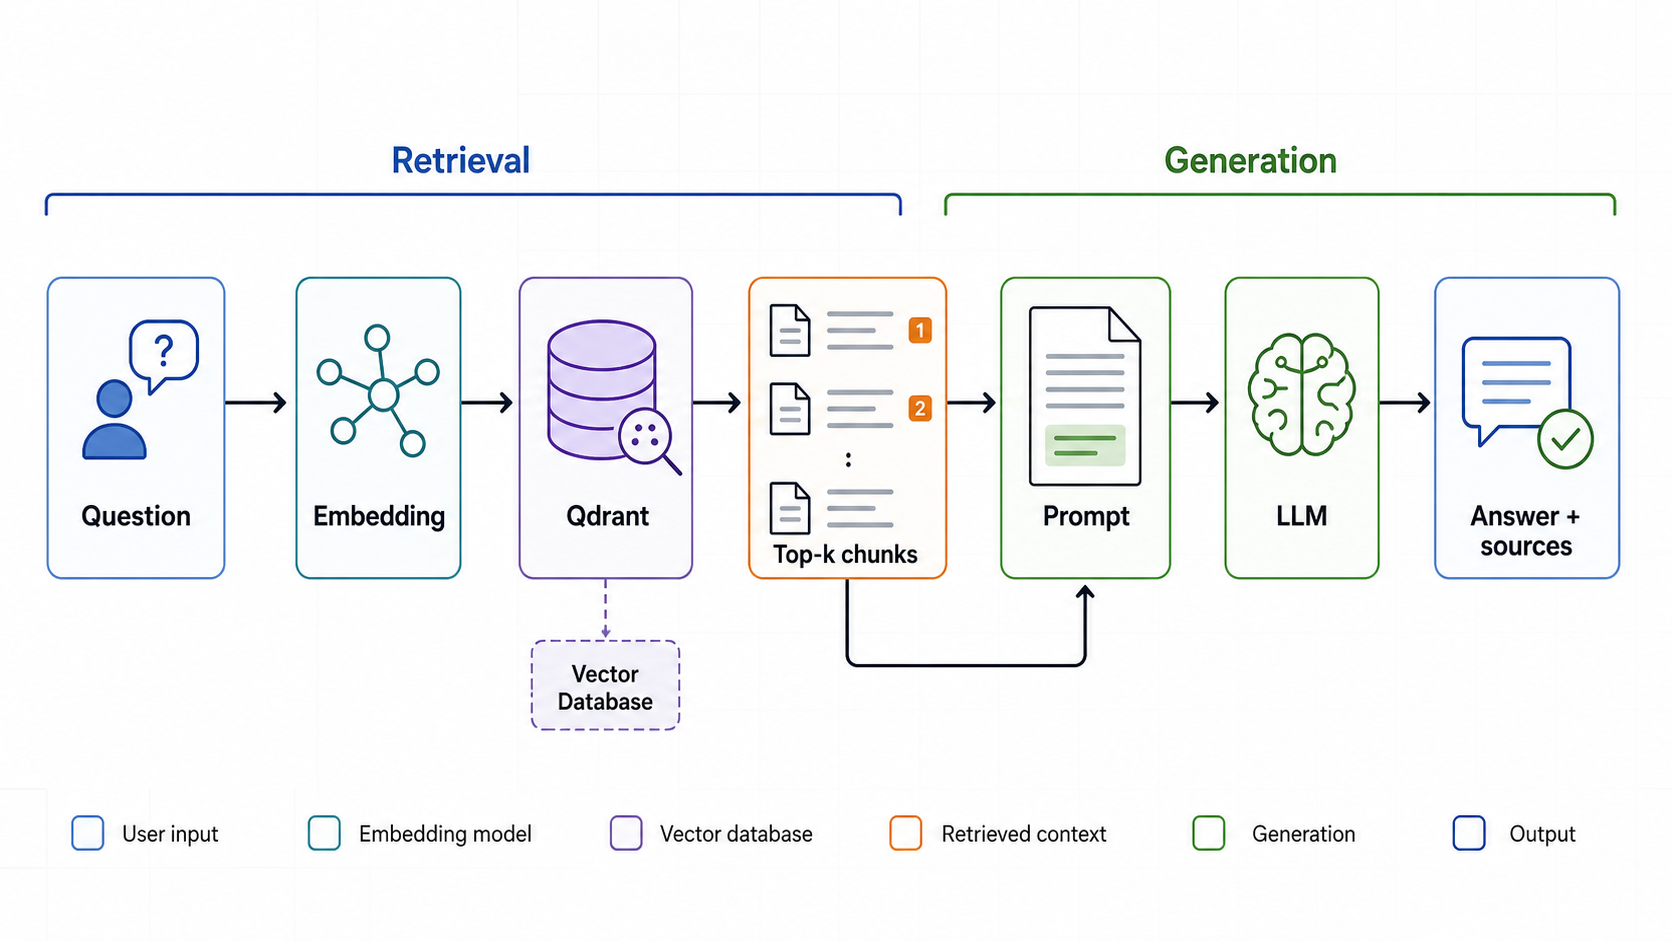
\includegraphics[width=\textwidth]{img/generated/rag_pipeline_overview.png}
\caption{Общая схема базового RAG-пайплайна}
\label{fig:rag-pipeline}
\end{figure}

На рисунке~\ref{fig:rag-pipeline} показано разделение RAG на retrieval-часть и generation-часть. Retrieval отвечает за нахождение фрагментов, а generation — за формирование связного ответа по найденному контексту. Важным свойством такой архитектуры является проверяемость: вместе с ответом могут возвращаться идентификаторы чанков и сведения об исходных документах.

\section{Выводы по главе}

Теоретическая основа MVP включает LLM, embedding-представления, векторный поиск и RAG. Векторная база данных используется для поиска релевантных фрагментов, а LLM — для формирования ответа по найденному контексту. Такая схема позволяет построить минимальный прототип без дообучения языковой модели и без усложнения retrieval-части.

%%% Local Variables:
%%% TeX-engine: xetex
%%% End:
